\documentclass[]{article}
\usepackage{lmodern}
\usepackage{amssymb,amsmath}
\usepackage{ifxetex,ifluatex}
\usepackage{fixltx2e} % provides \textsubscript
\ifnum 0\ifxetex 1\fi\ifluatex 1\fi=0 % if pdftex
  \usepackage[T1]{fontenc}
  \usepackage[utf8]{inputenc}
\else % if luatex or xelatex
  \ifxetex
    \usepackage{mathspec}
  \else
    \usepackage{fontspec}
  \fi
  \defaultfontfeatures{Ligatures=TeX,Scale=MatchLowercase}
\fi
% use upquote if available, for straight quotes in verbatim environments
\IfFileExists{upquote.sty}{\usepackage{upquote}}{}
% use microtype if available
\IfFileExists{microtype.sty}{%
\usepackage{microtype}
\UseMicrotypeSet[protrusion]{basicmath} % disable protrusion for tt fonts
}{}
\usepackage[unicode=true]{hyperref}
\hypersetup{
            pdfborder={0 0 0},
            breaklinks=true}
\urlstyle{same}  % don't use monospace font for urls
\usepackage{graphicx,grffile}
\makeatletter
\def\maxwidth{\ifdim\Gin@nat@width>\linewidth\linewidth\else\Gin@nat@width\fi}
\def\maxheight{\ifdim\Gin@nat@height>\textheight\textheight\else\Gin@nat@height\fi}
\makeatother
% Scale images if necessary, so that they will not overflow the page
% margins by default, and it is still possible to overwrite the defaults
% using explicit options in \includegraphics[width, height, ...]{}
\setkeys{Gin}{width=\maxwidth,height=\maxheight,keepaspectratio}
\IfFileExists{parskip.sty}{%
\usepackage{parskip}
}{% else
\setlength{\parindent}{0pt}
\setlength{\parskip}{6pt plus 2pt minus 1pt}
}
\setlength{\emergencystretch}{3em}  % prevent overfull lines
\providecommand{\tightlist}{%
  \setlength{\itemsep}{0pt}\setlength{\parskip}{0pt}}
\setcounter{secnumdepth}{0}
% Redefines (sub)paragraphs to behave more like sections
\ifx\paragraph\undefined\else
\let\oldparagraph\paragraph
\renewcommand{\paragraph}[1]{\oldparagraph{#1}\mbox{}}
\fi
\ifx\subparagraph\undefined\else
\let\oldsubparagraph\subparagraph
\renewcommand{\subparagraph}[1]{\oldsubparagraph{#1}\mbox{}}
\fi

% set default figure placement to htbp
\makeatletter
\def\fps@figure{htbp}
\makeatother


\date{}

\begin{document}

18/01/2017

Lezione ``Medicina di famiglia''

Dott. Stefano del Canale

Sbobinatore: Roberto Tozzi

\textbf{APPROPRIATEZZA PRESCRITTIVA NEL PAZIENTE ANZIANO (sezione)}

{[}Comparsata di Signorelli che fa un preambolo riguardante i moduli di
Medicina Generale, che alternano aspetti organizzativi del SSN con altri
di gestione clinica del paziente. La buona gestione di un paziente non
solo migliora la qualità della vita del paziente, ma fa anche bene al
sistema, perchè parte degli sprechi oggi sono legati alla gestione non
ottimale dei malati cronici.

Riguardo alla lezione di oggi, dice che, in seguito ad un'ispezione
europea per il controllo delle malattie infettive, è emerso che l'Italia
è tra i 3 paesi europei dei 27 che usano peggio gli antibiotici.{]}

Stamattina si parlerà di Farmacologia Clinica.

L'appropriatezza prescrittiva del paziente anziano è un progetto
dell'Ausl di Pr, che decorre dal 2007, in collaborazione con la
Jefferson University of Philadelphia.

La lezione si snoda attorno a 3 tematiche:

\begin{itemize}
\item
  Farmaci e Paziente Anziano
\item
  Progetto appropriatezza prescrittiva
\item
  De-Prescrizione

  Quando maneggiamo farmaci dobbiamo garantire efficacia di impiego e
  sicurezza del paziente. Secondo la WHO attualmente in Italia circa il
  20\% della popolazione è \textgreater{} di 65 anni (fascia tecnica per
  cui un individuo è definito anziano) e si stima che entro il 2030 il
  30\% della popolazione sarà costituita da anziani. Ciò fa avere
  un'idea precisa della tipologia di paziente che affrontiamo in
  ambulatorio o presso il proprio domicilio.

  \emph{1.PROBLEMA DEI FARMACI NEL PAZIENTE ANZIANO} (sottosezione)

  Il 95\% dei pazienti anziani ( \textgreater{}65 anni) in Italia usa
  almeno un farmaco all'anno.

  Il paziente anziano consuma mediamente 3 volte più farmaci e assorbe
  \emph{circa il 70\%} di tutte le risorse farmaceutiche. Usa spesso
  differenti farmaci contemporaneamente (perchè portatore cronico di
  diverse patologie) e presenta alterazioni fisiologiche dello
  ``handling''epatico e renale dei farmaci a cui consegue un'alterata
  farmacocinetica.

  \textbf{Limiti delle sperimentazioni pre-marketing dei farmaci} (lungo
  processo che può durare più di 10 anni e che consegna dalla molecola
  sperimentale a quella commercializzata e usata):
\end{itemize}

\begin{itemize}
\item
  ridotto numero di soggetti= impossibilità di scoprire reazioni avverse
  rare
\item
  protocolli sperimentali rigidi= esclusione di sottogruppi di
  popolazione
\item
  durata limitata= impossibilità di scoprire reazioni ritardate

  C'è tutto un mondo after-marketing che impatta il MMG nella pratica
  quotidiana.

  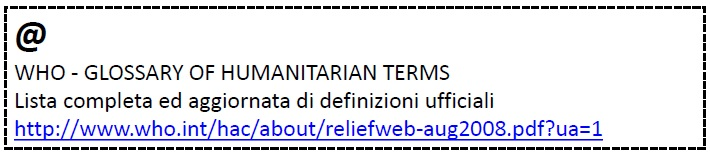
\includegraphics[width=3.98958in,height=3.33264in]{media/image1.wmf}

  Nel grafico sopra c'è un lavoro fatto su pazienti italiani, pubblicato
  sul New England Journal of Medicine nel 2012: paragone per ogni fascia
  di età tra i pazienti trattati attualmente con farmaci cardiovascolari
  e pazienti rispetto ai farmaci stessi reclutati in trials precedenti
  la commercializzazione. Più il pz è anziano, meno viene rappresentato
  nei trials e più consuma farmaci.

  \textbf{Adverse Drug Event (ADE)= Reazioni Avverse ai Farmaci}:
  secondo la WHO , si tratta di una reazione inaspettata che si possa
  presentare durante un trattamento farmacologico, che però non abbia
  necessariamente una relazione causale col trattamento stesso.

  2 tipologie di ADE:
\end{itemize}

\begin{itemize}
\item
  \textbf{prevenibili}: causate da errori medici nella prescrizione,
  dispensazione, somministrazione, monitoraggio del farmaco
\item
  \textbf{non prevenibili}: derivano dall'uso che il medico ne fa senza
  alcun errore nei passaggi precedenti

  Errori di prescrizione:

  - non considerare la presenza di controindicazioni

  - non sapere di reazioni sconosciute (Drug-to-Drug, Drug-to-Disease,
  Drug-to-Food)

  - eccessiva terapia farmacologica (polifarmaci)

  \textbf{Farmaci ed Anziani}: circa la metà dei decessi legati all'uso
  di farmaci avvengono in soggetti \textgreater{}65 anni. Negli USA il
  17\% dei ricoveri ospedalieri degli anziani è causato da ADEs.

  Infatti uno studio fatto proprio negli Stati Uniti, relativo al
  consumo di farmaci ad alto rischio ed interazioni farmaco-malattia
  testimonia che uno scorretto uso di farmaci ad alto rischio comporta
  una cascata di eventi che aumenta i costi sanitari.

  \emph{2. PROGETTO APPROPRIATEZZA PRESCRITTIVA} (sottosezione)

  \textbf{Gli obiettivi del ``Progetto Appropriatezza Prescrittiva} nel
  Paziente Anziano Ausl Pr 2007-2017''sono:
\end{itemize}

\begin{itemize}
\item
  sensibilizzare i MMG sul problema della prescrizione dei farmaci nel
  paziente anziano
\item
  migliorare la qualità delle prescrizioni
\item
  stimolare il confronto fra MMG e specialisti (ospedalieri e
  territoriali) per uniformare le prescrizioni

  \textbf{GAP (Gruppo Appropriatezza Prescrittiva)}: gruppo di medici
  ospedalieri e non, che aderiscono al Progetto e a cui, nel corso degli
  anni, sono stati sottoposti problemi che emergevano dalla letteratura,
  sull'utilizzo dei farmaci. Hanno stabilito criteri di
  inappropriatezza, secondo letteratura e criteri di Beers (oncologo,
  editor manuale Merk, si occupa di farmacologia clinica).

  \textbf{Criteri di in appropriatezza-Lista GAP}:
\end{itemize}

\begin{itemize}
\item
  farmaci che dovrebbero essere evitati: farmaci che la letteratura
  riporta ad alto rischio per l'anziani, esistono alternative più sicure
\item
  farmaci raramente appropriati: farmaci efficaci ma non di prima
  scelta, con un profilo rischio/beneficio e/o beneficio/costo non
  favorevole
\item
  farmaci da usare solo per indicazioni specifiche: farmaci che hanno
  alcune indicazioni, ma che spesso devono essere usati sotto stretto
  controllo; tali farmaci sono potenzialmente soggetti ad un uso non
  appropriato

  \textbf{Lista di farmaci potenzialmente inappropriati 2014}

  Ne sono state fatte 3 liste: 2012/13/14. Ovviamente da aggiornare. Per
  farmaci si intendono singoli farmaci o categorie. Sono inclusi anche
  limiti temporali (es. Aulin 2 vs 15-20 gg). Esempi:
\end{itemize}

\begin{itemize}
\item
  FANS
\item
  Nifedipina (dà crisi ipertensive)
\item
  Risparmiatori potassio (negli anziani, con riduzione della funzione
  renale, non si potrebbero usare dosi\textgreater{}25 mg/die)
\item
  Prazoli (insostituibili per la guarigione di un'ulcera peptica, per
  l'eradicazione di H.P., per la protezione in pz che devono prendere
  fans e grossi fattori di rischio; possono dare gravi effetti
  collaterali se si utilizzano in modo cronico e senza rivalutazione
  della terapia. Esempi di effetti collaterali: cala assorbimento di Ca,
  Mg, K, B12 e ciò comporta diminuzione della mineralizzazione ossea ed
  aumenta il rischio di fratture, oltre che anemia; aumenta l'incidenza
  di demenze e di IRC e IRA. In questi casi si torna ai vecchi H2
  recettori, meno efficaci, ma che danno meno effetti collaterali)
\item
  Antiaritmici, es. Amiodarone, usato tantissimo in Italia, no in USA,
  viene usato solo per gravi aritmie ventricolari

  
\includegraphics[width=5.19722in,height=2.60347in]{media/image2.wmf}

  Il grafico qui sopra mostra l'inappropriatezza farmaci somministrati a
  Pr: 25\% (nella nostra AUSL 1 anziano su 4 riceve farmaci che non
  dovrebbe usare)

  
\includegraphics[width=5.40556in,height=4.06181in]{media/image3.wmf}

  \emph{2.1 FARMACI A CARICO DEL SSN CHE DOVREBBERO ESSERE EVITATI}
  (sotto sottosezione)

  L'impiego di \textbf{FANS} per un periodo maggiore di 15 gg dovrebbe
  essere evitato, in quanto in pazienti anziani gli effetti avversi di
  tali farmaci possono esacerbarsi fino ad includere tossicità renale e
  cardiovascolare (incremento della pressione) e rischio elevato di
  emorragie gastriche.

  Se vi è necessità di terapia antidolorifica prolungata per patologie
  artroreumatiche (spondilite anchilosante o artrite reumatoide) e il
  paracetamolo non risulta sufficiente nella gestione della
  sintomatologia, si può usare in alternativa e in ordine crescente di
  potenza:
\end{itemize}

\begin{enumerate}
\def\labelenumi{\arabic{enumi}.}
\item
  Codeina + Paracetamolo
\item
  Tramadolo, da solo o con paracetamolo
\item
  Ossicodone, da solo o con paracetamolo
\item
  Morfina solfato

  Nella terapia prolungata del dolore neoplastico si propone l'uso di:
\end{enumerate}

\begin{enumerate}
\def\labelenumi{\arabic{enumi}.}
\item
  Tramadolo
\item
  Ossicodone
\item
  Morfina solfato
\item
  Buprenorfina
\item
  Fentanyl

  \emph{2.2 FARMACI A CARICO DEL SSN APPROPRIATI SOLO PER ALCUNE
  CONDIZIONI} (sotto sottosezione)

  \textbf{L'amiodarone} è associato a problemi di intervalli QT e
  rischio di provocare torsioni di punta. Presenta scarsa maneggevolezza
  terapeutica, specialmente nell'anziano, oltre a tossicità polmonare,
  epatica, oculare, tiroidea e polineuropatie.

  Esso rappresenta la prima scelta nei pz in cui oltre alla
  fibrillazione atriale (FA) vi siano anche danni strutturali cardiaci
  quali:
\end{enumerate}

\begin{itemize}
\item
  FA + ipertensione con ipertrofia ventricolare sx
\item
  FA + coronaropatia
\item
  FA + insufficienza cardiocircolatoria

  Il dosaggio massimo nell'anziano è di 100mg/die; se somministrato in
  quei pazienti anziani che corrispondono ai criteri di scelta, è
  comunque necessaria una valutazione preliminare all'inizio della
  terpaia di funzione epatica, tiroidea, polmonare. Nei pz in terapia
  con Warfarin, il dosaggio di quest'ultimo va ridotto del 25\%
  all'inizio della terapia con amiodarone.

  Pur essendo superiore come attività antiaritmica e
  \textbf{Propafenone} e \textbf{Sotalolo} è considerato farmaco di
  seconda scelta nella FA dell'anziano senza danni strutturali cardiaci

  \emph{2.3 Sessioni informative/formative su specifici farmaci/classi
  di farmaci inappropriati 2012-2016 (}sotto sottosezione)

  Già effettuate

  -antinfiammatori

  -inibitori di pompa

  -antiaritmici

  -antipsicotici

  Nel prossimo biennio, un focus su

  -antidepressivi

  -ipoglicemizzanti

  L'88\% dei medici crede di prescrivere correttamente i farmaci; nella
  realtà la maggior parte dei medici non si informa correttamente.

  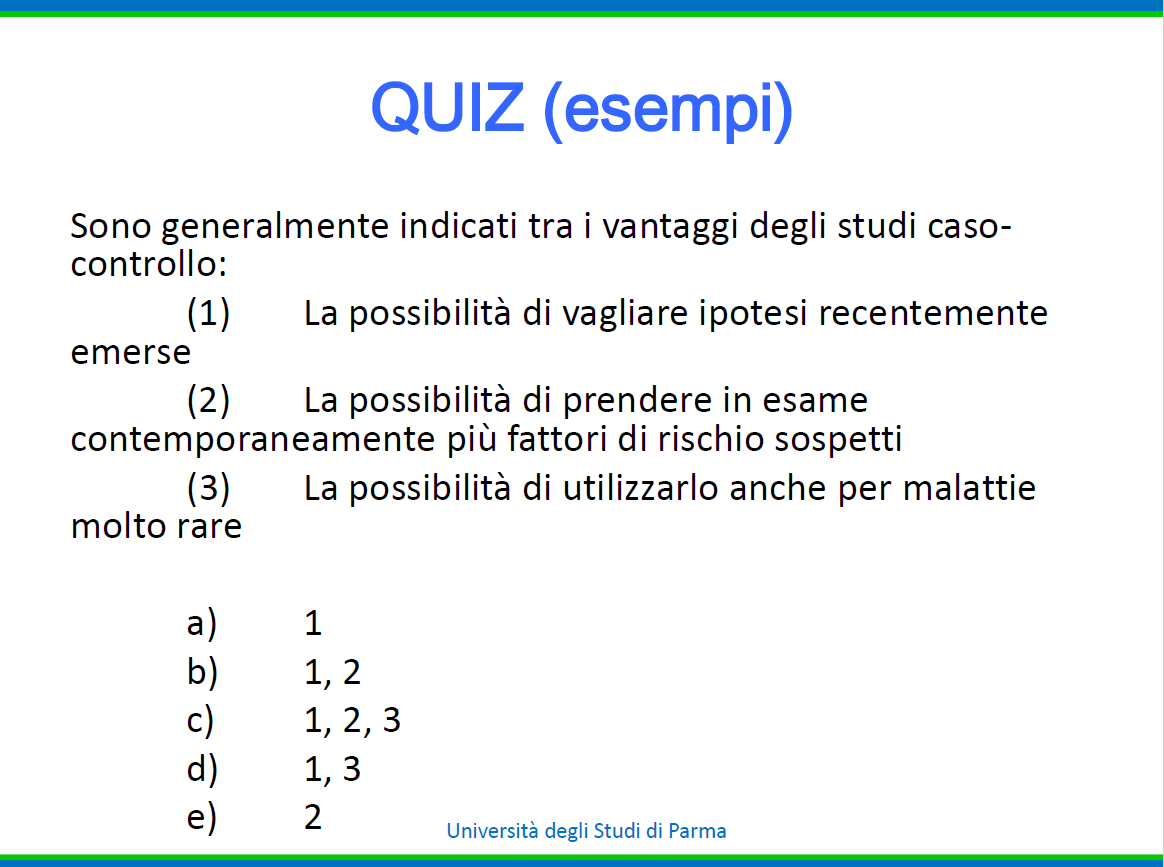
\includegraphics[width=5.32222in,height=2.14514in]{media/image4.wmf}

  N.B. Tutte le terapie dovrebbero essere rivalutate annualmente dal MMG

  \emph{3.DEPRESCRIZIONE} (Sottosezione)

  Processo sistematico di identificazione e discontinuazione di farmaci
  in circostanze in cui gli effetti negativi ne superano i benefici, sia
  attuali sia potenziali, e questo all'interno del contesto degli
  obiettivi di cura, alla aspettativa di vita, ai valori e alle
  preferenze del singolo paziente. (Scott IA et al. JAMA Internal
  Medicine, 2015)

  Non è un processo che porta a negare un trattamento efficace a quel
  paziente che ne può beneficiare. E' un processo necessario ad
  assicurare che il paziente non riceva trattamenti che non solo non
  hanno benefici certi, ma che con molta probabilità possono avere
  effetti negativi.

  \textbf{Motivi di deprescrizione}:
\end{itemize}

\begin{itemize}
\item
  Mancanza di efficacia
\item
  Probabile o certa reazione avversa da farmaci
\item
  Non-aderenza
\item
  Risoluzione del problema medico
\item
  Insorgenza di controindicazioni
\item
  Interazione fra farmaci
\item
  Aspettativa di vita (eprognosis for elders)

  \textbf{Barriere alla deprescrizione: medico}
\end{itemize}

\begin{itemize}
\item
  Complessità clinica del paziente
\item
  Limiti di tempo della visita medica
\item
  Frammentazione della continuità di cure (multi-prescrittori)
\item
  Mancanza di evidenza sull'efficacia/eventi avversi nella
  continuazione/deprescrizione dei farmaci
\item
  Inconsistenza degli obiettivi di cura
\item
  Attitudine a prescrivere piuttosto che a de prescrivere
\item
  Utilizzo razionale delle raccomandazioni delle linea guida

  \textbf{Barriere alla deprescrizione: paziente}
\end{itemize}

\begin{itemize}
\item
  Convinzione che il farmaco porti a benefici
\item
  Paura degli effetti del processo di de prescrizione
\item
  Paura del peggioramento della condizione medica
\item
  Precedente esperienza negativa di cessazione del farmaco
\item
  Influenza dei familiari caregivers/di opinioni ``qualificate''

  \textbf{Algoritmi di deprescrizione specifici per classi di farmaci,
  es Inibitori della Pompa Protonica (PPI).}

  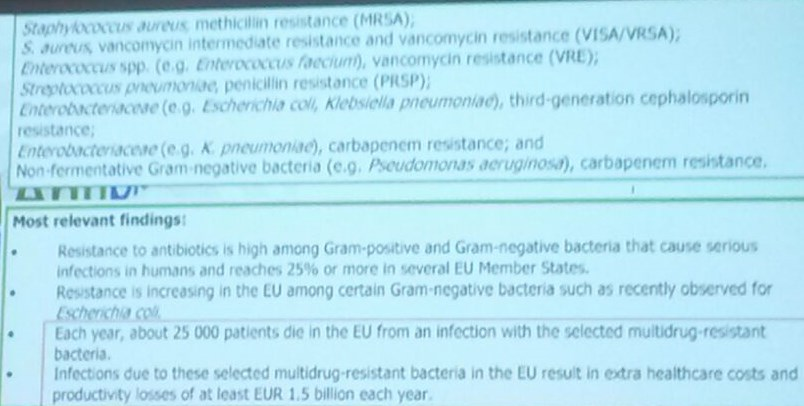
\includegraphics[width=5.97847in,height=4.12431in]{media/image5.wmf}

  Se si sospendono i PPI si deve monitorare il pz per un paio di
  settimane per vedere se ha sintomi da rebound.
\end{itemize}

\end{document}
